\chapter{Результаты и обсуждения}


\section{Ответы на вопросы исследования}

Мы получили следующие ответы на вопросы исследования, поставленные в разделе \hyperref[intro-questions]{Вопросы исследования}.

1. Как несколько агентов могут научиться сотрудничать друг с другом во время обучения в определенных игровых сценариях?

Ответ: во время обучения, для изучения оптимальной политики сотрудничества, агенты должны принимать во внимание совместные наблюдения и совместные действия всех агентов.

2. Может ли после обучения появиться язык между агентами в определенных игровых сценариях?

Ответ: да, когда обучение сходится, композиционный язык у агентов возникает.

3. Как можно оптимизировать и ускорить процесс обучения?

Ответ: для ускорения обучения существуют разные методы и приемы. В этой работе мы пробовали применить некоторые из них, такие как: обучение с общим мозгом, декомпозированное вознаграждение, обучение по учебной программе.

\newpage


\section{Сетевая архитектура}

В таблице \taref{tab-algs-application} показано применение различных сетевых архитектур к различным игровым сценариям.

\begin{table}[t!]
    \centering\small
    \caption{Подходящие сетевые архитектуры для разных игровых сценариев}
    \label{tab-algs-application}
    \begin{tabular}{|l|l|l|l|l|l|}
        \hline
        & MADDPG & MADDPG с одним мозгом & Декомпозированная награда \\
        \hline
        Speaker Listener    & v      & x                     & x                         \\ \hline
        Simple Reference    & v      & v                     & v                         \\ \hline
        World Communication & v      & x                     & v                         \\ \hline
        Simple Tag          & v      & v                     & x                         \\ \hline
    \end{tabular}
    \normalsize% возвращаем шрифт к нормальному
\end{table}

Такие сценарии, как \textit{Simple Speaker Listener} с двумя агентами, разделяющими глобальное вознаграждение, но обладающими разными наблюдениями и пространствами действий, могут использовать только стандартный MADDPG. Поскольку агенты функционируют по-разному, им необходимо искать различные оптимальные политики для своих ролей в игре.

Такие сценарии, как \textit{Simple Reference}, где два агента совместно получают глобальное вознаграждение, имеют одно и то же пространство действий и пространство наблюдений могут работать со стандартным MADDPG, а также эти сценарии могут использовать \textit{общий мозг}, или \textit{декомпозированную награду}.

Наиболее эффективной архитектурой являются использование сети с \textit{общим мозгом}, поскольку при этом обучается меньшее количество сетей. Это значительно повышает эффективность обучения игровых сценариев, которые можно адаптировать к сетям с \textit{общим мозгом}.

В сценарии \textit{Simple Tag} агенты из одной «команды» так же имеют одинаковые пространства наблюдений и действий. Мы применили здесь отдельный набор \textit{акторов-критиков} для \textit{преследователей} и отдельный - для \textit{жертв}. Общение в этом сценарии отсутствует, поэтому \textit{декомпозированная награда} здесь не имеет смысла. Этот сценарий был выбран для сравнения стандартного MADDPG с MADDPG с \textit{одним мозгом}.

\newpage


\section{Сценарии}

Первые два сценария не предполагают конкуренции и не требуют большого количества шагов для достижения результата, поэтому их эпизоды ограничены 25 шагами. 

Эксперименты со вторыми двумя сценариями мы решили дать агентам возможность двигаться подольше и ограничили их длительность 150 шагами. Это замедлило обучение, но иначе невозможно обучить агентам сколько-нибудь сложномым тактикам.

Во всех экспериментах проигрывалось 20000 эпизодов.

\subsection{Сценарий 1. Simple Speaker Listener}

Сходимость этого сценария становится возможной, когда \textit{говорун} сообщает правильные целевые ориентиры и \textit{слушатель} достигает их. В проведённых экспериментах агенты обучались с помощью алгоритмов MADDPG и DDPG.

\begin{figure}[ht!]
    \center
    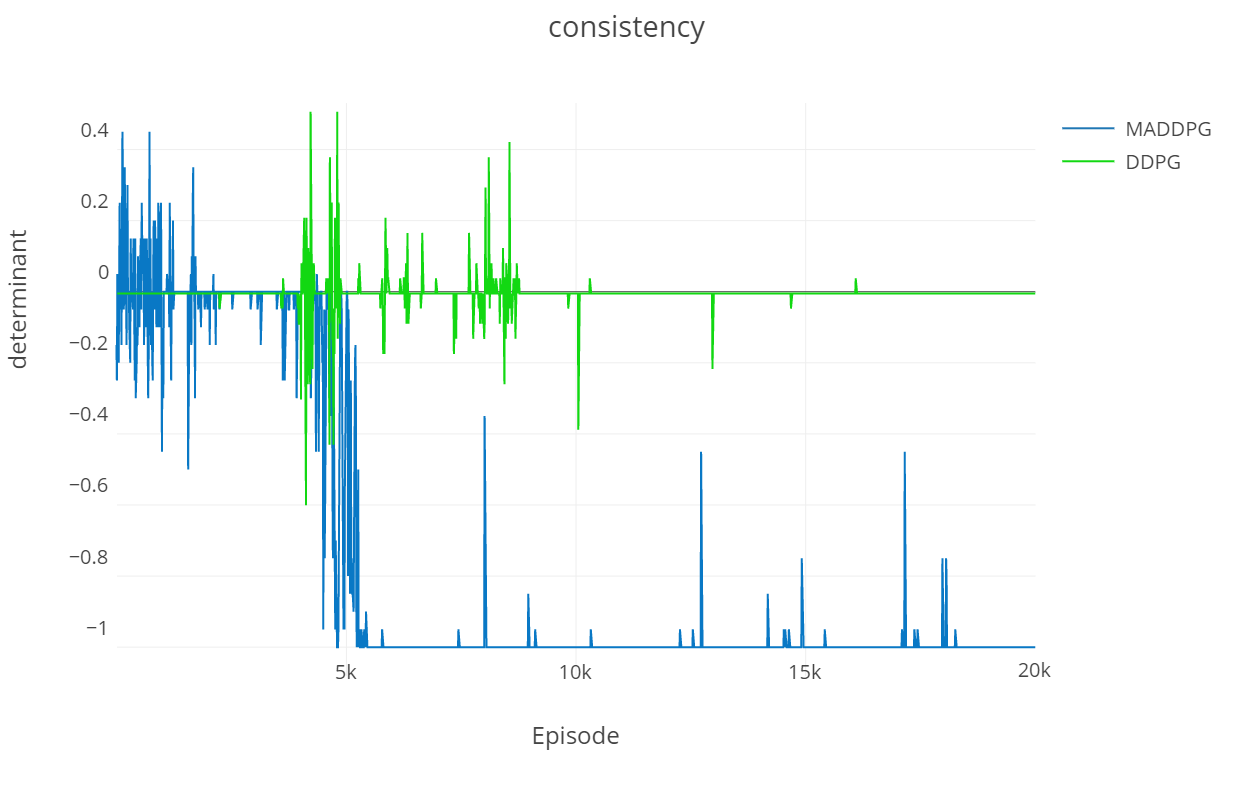
\includegraphics [scale=0.38] {my_folder/images/ch5/ssl-comm.png}
    \caption{График согласованности коммуникаций \textit{говоруна} в сценарии \textit{Simple Speaker Listener}}
    \label{fig:result-ssl-comm}
\end{figure}

Мы построили графики согласованности коммуникаций и вознаграждений для двух агентов в сценарии \textit{Simple Speaker Listener}, которые представлены на \firef{fig:result-ssl-comm} и \firef{fig:result-ssl-rew}. На этих графиках синяя кривая - это результат обучения MADDPG, а зелёная - DDPG.

График на \firef{fig:result-ssl-comm} показывает сходимость консистентности действий общения для \textit{говоруна}, как описано в разделе \hyperref[exp-ssl]{Сценарии}. Этот график показывает, что сходится он только для MADDPG. Это указывает на то, что \textit{говорун}, обученный MADDPG, может постоянно интерпретировать ориентир в одной и той же кодировке, в то время как \textit{говорун}, обученный DDPG, не может поддерживать консистентное общение.

\begin{figure}[ht!]
    \center
    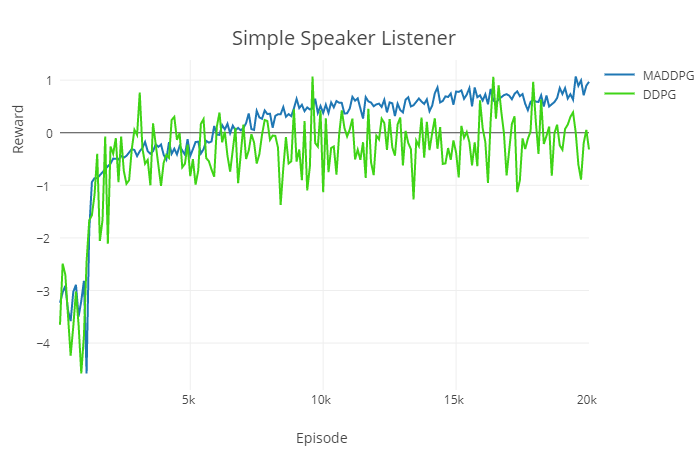
\includegraphics [scale=0.60] {my_folder/images/ch5/ssl-rew.png}
    \caption{График среднего вознаграждения для двух агентов в сценарии Simple Speaker Listener. Результаты обучения по алгоритму MADDPG и DDPG}
    \label{fig:result-ssl-rew}
\end{figure}

График на \firef{fig:result-ssl-rew} показывает среднее вознаграждение, которое агенты получили в конце каждого эпизода. Из этого графика видно, что вознаграждение, полученное агентами, обученными DDPG, ниже, чем агентами, обученными MADDPG.

\begin{figure}[ht!]
    \center
    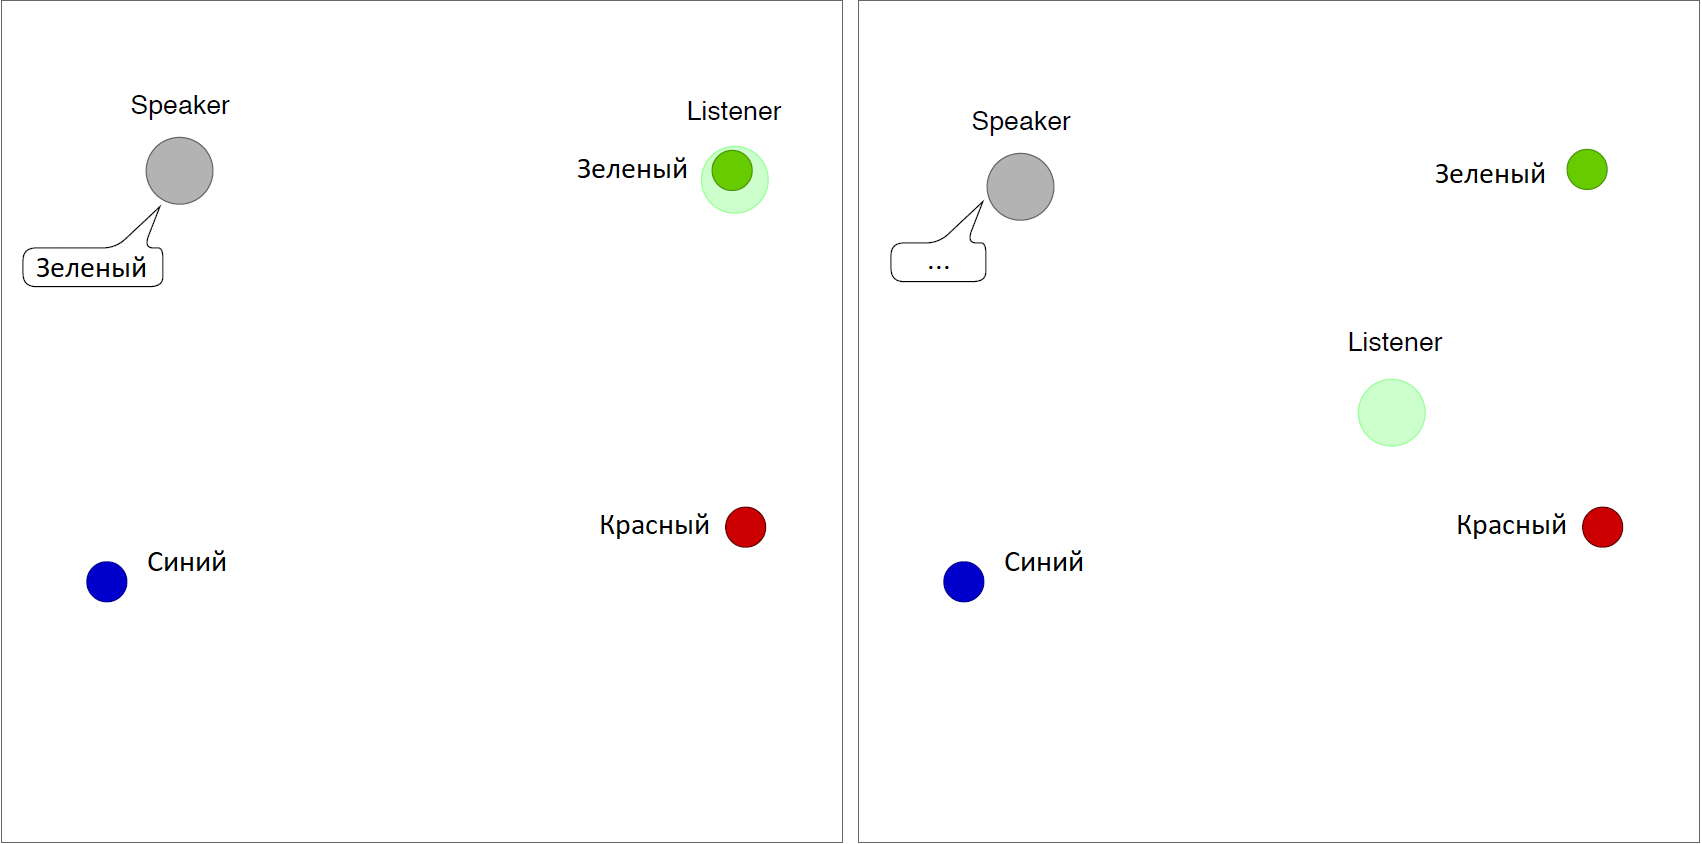
\includegraphics [scale=0.45] {my_folder/images/ch5/results-ssl-conv-non-conv.png}
    \caption{На левой стороне: \textit{говорун} произносит корректное высказывание, \textit{слушатель} перемещается к цели. Справа: коммуникационное действие отсутствует, и \textit{слушатель} застревает между тремя ориентирами (видимо, в попытке минимизировать расстояние до каждого из них)}
    \label{fig:result-conv-non-conv}
\end{figure}

Агенты, обученные DDPG, предпринимают действия, не имея полного наблюдения за состоянием окружающей среды и политикой других агентов. Они не в состоянии изучить политику оптимального взаимодействия друг с другом

На \firef{fig:result-conv-non-conv} показан скриншот при сходимости и не сходимости \textit{Simple Speaker Listener}.

\subsection{Сценарий 2. Simple Reference}

Сценарий \textit{Simple Reference} сходится, когда агенты правильно перемещаются к своим собственным целевым ориентирам. На \firef{fig-intro-sr} показан скриншот поведения агентов после схождения сценария \textit{Simple Reference}. В проведённых экспериментах агенты тренировались алгоритмами DDPG и MADDPG.

\begin{figure}[ht!]
    \center
    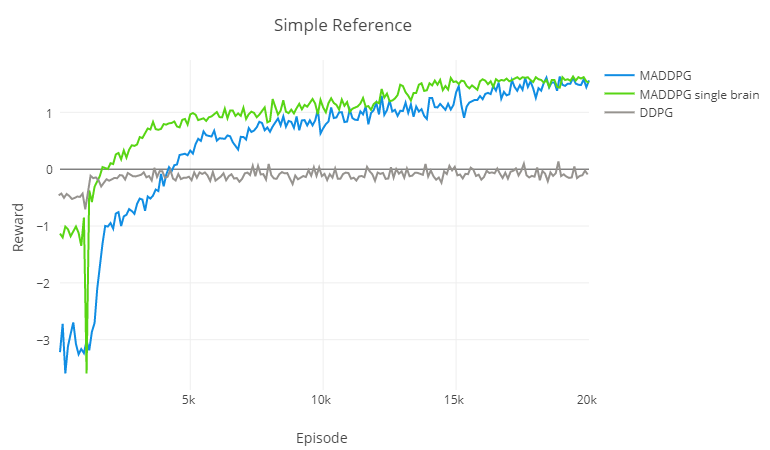
\includegraphics [scale=0.6] {my_folder/images/ch5/sr-rew.png}
    \caption{График среднего вознаграждения для двух агентов в сценарии \textit{Simple Reference}. Результаты обучения по алгоритму MADDPG, MADDPG с одним мозгом и DDPG}
    \label{fig:result-sr-rew}
\end{figure}

\begin{figure}[ht!]
    \center
    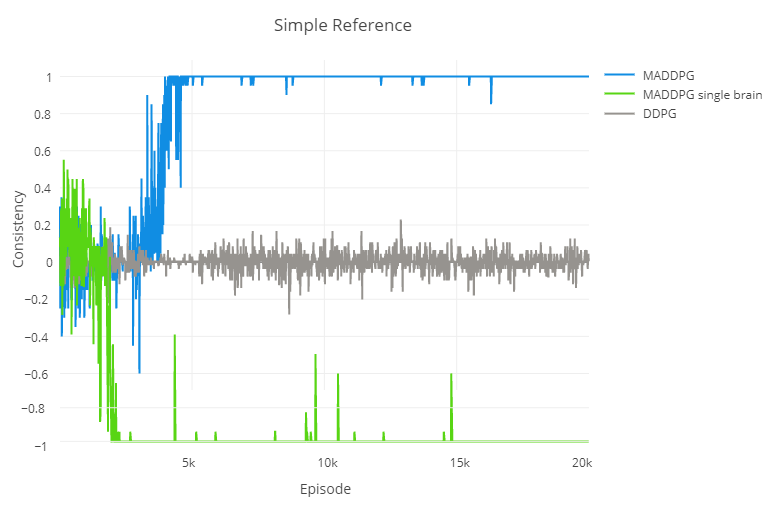
\includegraphics [scale=0.6] {my_folder/images/ch5/sr-comm.png}
    \caption{Графики согласованности взаимодействия для двух агентов в сценарии \textit{Simple Reference}. Результаты обучения по алгоритму MADDPG, MADDPG с одним мозгом и DDPG}
    \label{fig:result-sr-comm}
\end{figure}

Был построен график вознаграждения для двух агентов, который представлен на \firef{fig:result-sr-rew}. На этом графике синяя кривая~--- результат, обученный MADDPG, зелёная~--- одним мозгом, а серая~--- DDPG.

Агенты, обученные с помощью DDPG, получают меньшее вознаграждение, чем агенты MADDPG и его варианты. Также из рендеринга игры видно, что агенты DDPG блуждают среди ориентиров, не зная, какой из них является правильной целью.

Графики на \firef{fig:result-sr-comm} показывают согласованность действий общения. Для MADDPG и его варианта средний детерминант стремится к 1 или -1. Это указывает на то, что агенты, обученные с помощью этих алгоритмов, могут общаться согласованно. Для агентов, обученных DDPG, значение стремится к 0, это иллюстрируют, что они не могут корректно сообщать цели.

В процессе выполнения многочисленных экспериментов можно было наблюдать, что полная несходимость всегда сопровождается тем, что агенты, не способны дифференцировать и сообщать правильные ориентиры друг другу. То же справедливо и для частичной сходимости, когда агенты могут перемещаться только к тем ориентирам, которые правильно сообщены другими агентами, см. \firef{fig:result-sr-non-convergency}. Это также показывает, что агентам для достижения целей необходимо сотрудничать как в физических, так и в коммуникационных действиях.

\begin{figure}[ht!]
    \center
    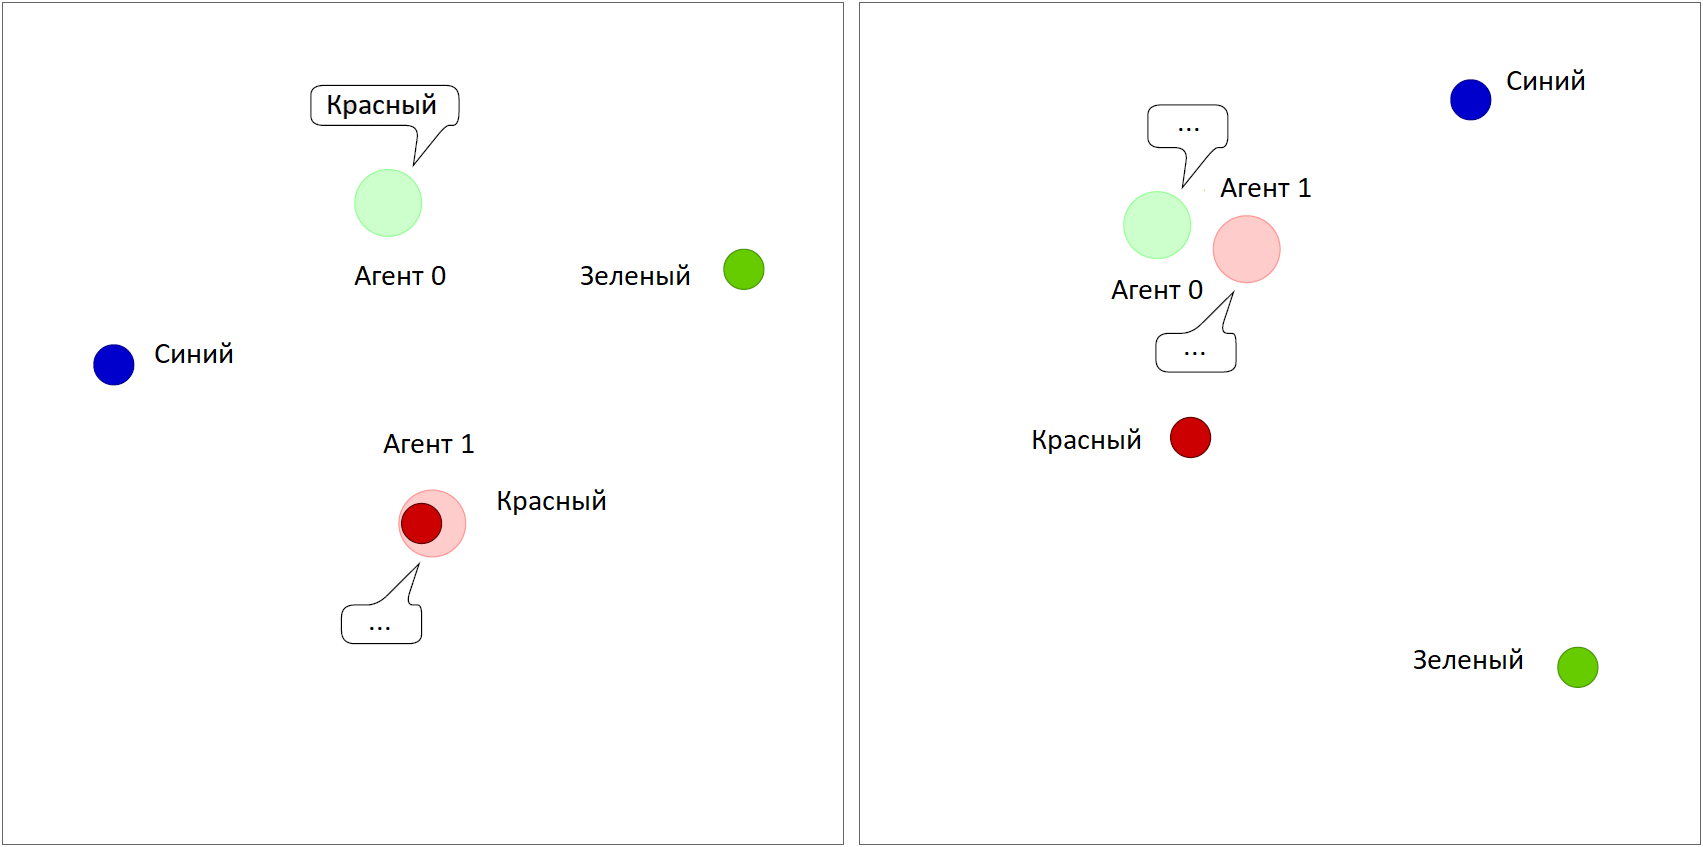
\includegraphics [scale=0.45] {my_folder/images/ch5/results-sr-non-convergency.png}
    \caption{Частичная сходимость с левой стороны: один агент перемещается к цели, а другой ждёт между ориентирами. Несходимость на правой стороне заканчивается тем, что оба агента не знают, куда двигаться и ждут между ориентирами}
    \label{fig:result-sr-non-convergency}
\end{figure}

Наконец, между агентами возникает язык. Проведённые эксперименты показали, что при каждой тренировке агенты по-разному интерпретируют ориентиры. Например, после одной тренировки красный ориентир может выглядеть как ${[1; 0; 0]}$, а после другой~--- как ${[0; 1; 0]}$ или ${[0; 0; 1]}$.

\begin{table}[t!]
    \centering\small
    \caption{Среднее время, потраченное на обучение с различными алгоритмами в 20000 эпизодах}
    \label{tab-sr-time}
    \begin{tabular}{|l|l|l|l|l|l|}
        \hline
        & DDPG           & MADDPG          & MADDPG с одним мозгом \\
        \hline
        Время, 20000 эпизодов & 698 $\pm$ 58~с & 820 $\pm$ 98~с & 635 $\pm$ 45~с       \\ \hline
    \end{tabular}
    \normalsize% возвращаем шрифт к нормальному
\end{table}

В \taref{tab-sr-time} показано время, затраченное на обучение по сценарию \textit{Simple Reference} с разными алгоритмами.

\subsection{Сценарий 3: Simple World Communication}

Мы построили графики вознаграждений и согласованности коммуникаций для двух преследователей и одной жертвы в сценарии \textit{Simple World Communication}, которые представлены на \firef{fig:result-swc-rew} и \firef{fig:result-swc-comm}. На этих графиках зеленая кривая - это результат обучения MADDPG, а серая - DDPG. Все они обучены по 20000 эпизодов.

\begin{figure}[ht!]
	\center
	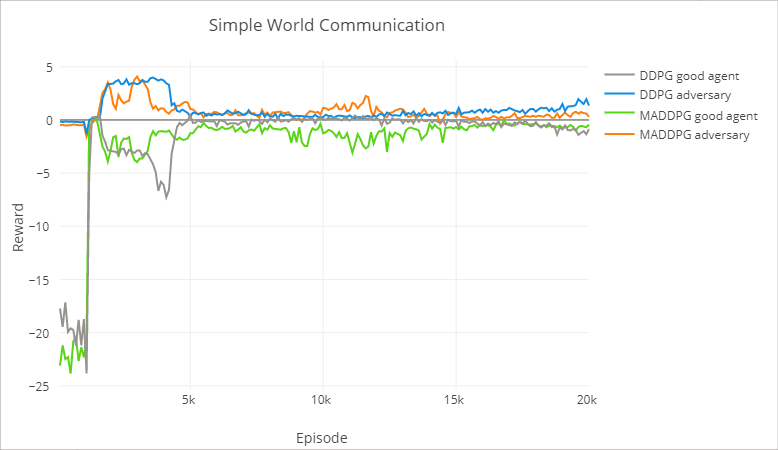
\includegraphics [scale=0.6] {my_folder/images/ch5/swc-rew.png}
	\caption{Среднее вознаграждение преследователей и жертвы с алгоритмами DDPG и MADDPG.}
	\label{fig:result-swc-rew}
\end{figure}

\begin{figure}[ht!]
	\center
	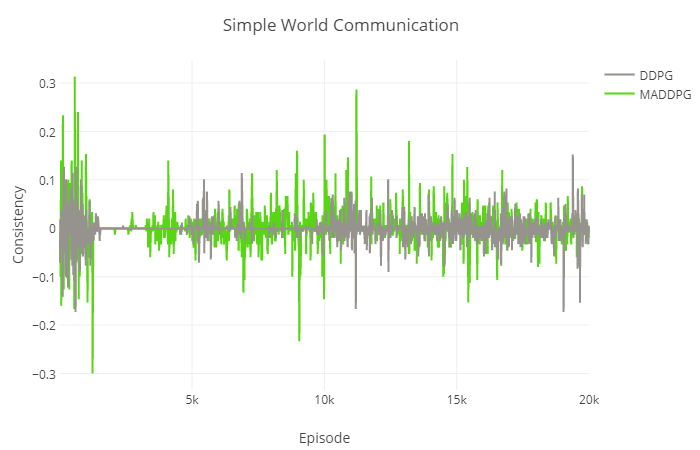
\includegraphics [scale=0.6] {my_folder/images/ch5/swc-comm.png}
	\caption{График консистентности действий коммуникации для алгоритмов DDPG и MADDPG.}
	\label{fig:result-swc-comm}
\end{figure}

К сожалению, из-за ограниченности времени и вычислительных ресурсов, нам не удалось добиться сходимости консистентности действий общения в этом сценарии, это видно на \firef{fig:result-swc-comm}. Из графика видно, что отклонения от нуля больше в случае MADDPG, но этого оказалось недостаточно для того, чтобы «закрепить результат», научиться преследователю использовать получаемые сигналы лидера так, чтобы улучшить общее вознаграждение.

В следствие чего, результаты алгоритма MADDPG ничем не выделяются по сравнению с DDPG, это можно видеть на \firef{fig:result-swc-rew}.

Так же, в этом сценарии трудно установить «конец игры», когда цель достигнута, так как во время обучения агенты обоих команд постепенно действуют все более адекватно, однако это трудно увидеть, на графике среднего вознаграждения. То преследователи изобретают более-менее эффективную тактику, и получают большую награду, то жертва обучается на своих ошибках и начинает учитывать это. Однако, на рендеринге можно видеть, что и преследователи, и жертва ведут себя вполне адекватно. Преследователи догоняют жертву, жертва убегает и, по возможности, стремиться к еде.

Скорее всего, если обучать модель дольше, мы бы увидели более сложные и согласованные действия преследователей.

\subsection{Сценарий 4: Simple Tag}

Как уже упоминалось \hyperref[exp-st]{выше}, этот сценарий не подразумевает коммуникационных действий. Но он был выбран нами, так как он достаточно сложный, и при этом агенты из одной команды имеют одинаковые пространства наблюдения и действий, что позволяет применить вариант алгоритма MADDPG с общим мозгом.

\paragraph{Двое против одного.}

Мы поставили эксперимент с двумя преследователями и одной жертвой.

На \firef{fig-st-reward-ad} и \firef{fig-result-st-reward-ag} изображены графики средней награды преследователей и жертв. Видно, что графики симметричны. Когда преследователи выучиваются двигаться в нужном направлении и понимают, что нужно гонятся за жертвой, они получают большую награду, а жертва меньшую. После чего, жертва выучивается убегать от преследователей - тогда её награда растёт, а награда преследователей снижается. Так же, как и в \hyperref[exp-results-svc]{предыдущем сценарии}.

\begin{figure}[!htbp]
    \adjustbox{minipage=1.3em,valign=t}{\subcaption{}\label{fig-st-reward-ad}}%
    \begin{subfigure}[t]{\dimexpr.5\linewidth-1.3em\relax} %разрешили выделить 0,5 стр в ширину на рисунок
        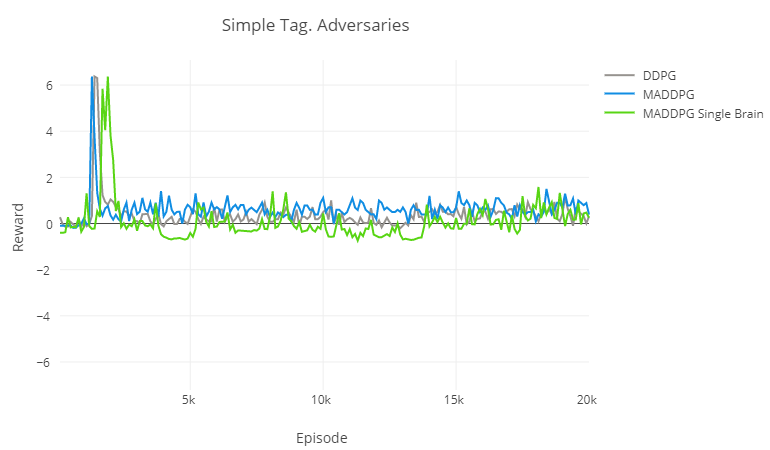
\includegraphics[height=0.19\textheight,valign=t]{my_folder/images/ch5/st-reward-ad.png} %высоту рисунка выставили как 0,3 от высоты наборного поля
    \end{subfigure}
    %	\hfill %выровнять по ширине
    \adjustbox{minipage=1.3em,valign=t}{\subcaption{}\label{fig-result-st-reward-ag}}%
    \begin{subfigure}[t]{\dimexpr.5\linewidth-1.3em\relax}%разрешили выделить 0,5 стр в ширину на рисунок
        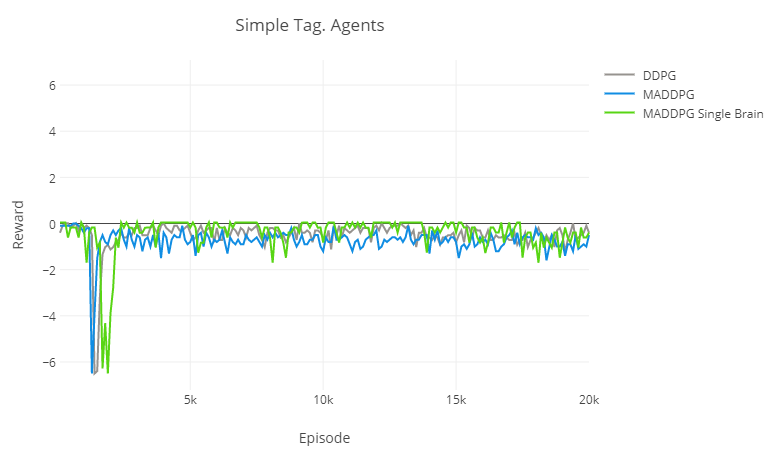
\includegraphics[height=0.19\textheight,valign=t]{my_folder/images/ch5/st-reward-ag.png}%высоту рисунка выставили как 0,3 от высоты наборного поля
    \end{subfigure}
    \captionsetup{justification=centering} %центрировать
    \caption{Награда с применением алгоритма DDPG, MADDPG, MADDPG с общим мозгом: {\itshape a} --- \textit{преследователей}; {\itshape b}~--- \textit{жертв}}\label{fig:spbpu_main_bld-two-photos}
\end{figure}

В \taref{tab-st-time} указано время, затраченное на обучение в данной конфигурации для разных алгоритмов.

\begin{table}[t!]
    \centering\small
    \caption{Среднее время, потраченное на обучение с различными алгоритмами в 20000 эпизодов. 2 преследователя, 1 жертва.}
    \label{tab-st-time}
    \begin{tabular}{|l|l|l|l|l|l|}
        \hline
        & DDPG       & MADDPG      & MADDPG с одним мозгом \\
        \hline
        Время, 20000 эпизодов & 7ч. 46мин. & 10ч. 24мин. & 3ч. 42мин.            \\ \hline
    \end{tabular}
    \normalsize% возвращаем шрифт к нормальному
\end{table}

\paragraph{Четверо против двоих.}

Так же, на этом сценарии мы поставили эксперименты с более сложными настройками - 4 \textit{преследователя} и 2 \textit{жертвы}.

\begin{figure}[!htbp]
    \adjustbox{minipage=1.3em,valign=t}{\subcaption{}\label{fig-result-st-4vs2-ddpg}}%
    \begin{subfigure}[t]{\dimexpr.5\linewidth-1.3em\relax} %разрешили выделить 0,5 стр в ширину на рисунок
        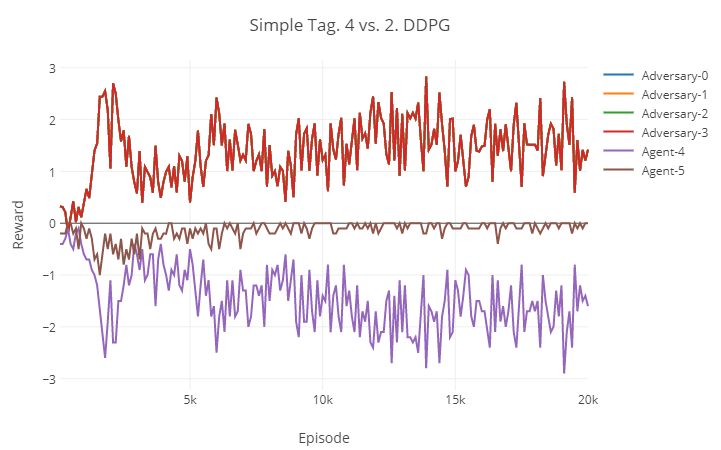
\includegraphics[height=0.20\textheight,valign=t]{my_folder/images/ch5/st-4vs2-ddpg.png} %высоту рисунка выставили как 0,3 от высоты наборного поля
    \end{subfigure}
    %	\hfill %выровнять по ширине
    \adjustbox{minipage=1.3em,valign=t}{\subcaption{}\label{fig-result-st-4vs2-maddpg}}%
    \begin{subfigure}[t]{\dimexpr.5\linewidth-1.3em\relax}%разрешили выделить 0,5 стр в ширину на рисунок
        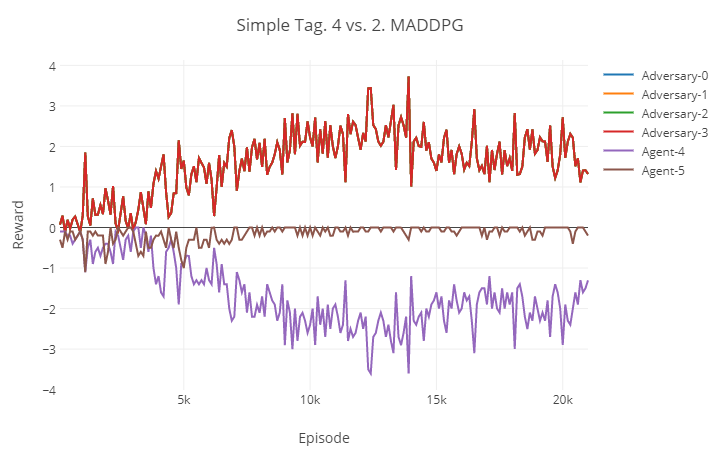
\includegraphics[height=0.20\textheight,valign=t]{my_folder/images/ch5/st-4vs2-maddpg.png}%высоту рисунка выставили как 0,3 от высоты наборного поля
    \end{subfigure}
    \adjustbox{minipage=1.3em,valign=t}{\subcaption{}\label{fig-result-st-4vs2-maddpg-sb}}%
    \begin{subfigure}[t]{\dimexpr.5\linewidth-1.3em\relax}%разрешили выделить 0,5 стр в ширину на рисунок
        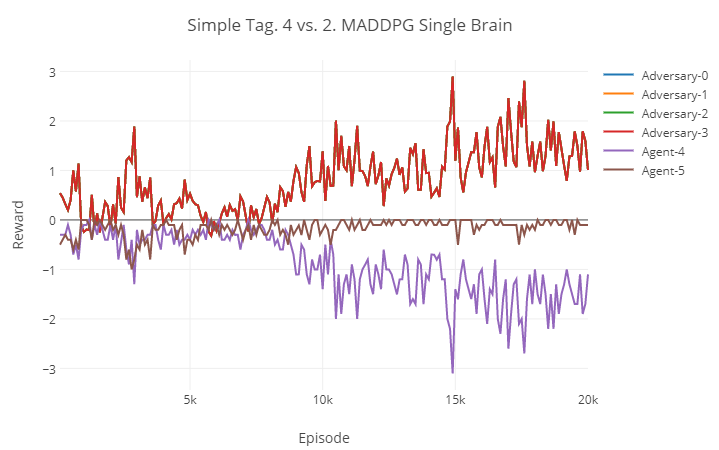
\includegraphics[height=0.20\textheight,valign=t]{my_folder/images/ch5/st-4vs2-maddpg-sb.png}%высоту рисунка выставили как 0,3 от высоты наборного поля
    \end{subfigure}
    \captionsetup{justification=centering} %центрировать
    \caption{Награда каждого из 6 агентов с применением алгоритма: {\itshape a} --- DDPG; {\itshape b}~--- MADDPG; {\itshape c}~--- MADDPG с общим мозгом}\label{fig:spbpu_main_bld-two-photos}
\end{figure}

На \firef{fig-result-st-4vs2-ddpg}, \firef{fig-result-st-4vs2-maddpg} и \firef{fig-result-st-4vs2-maddpg-sb} изображены графики средней награды преследователей и жертв.

В \taref{tab-st-4vs2-time} указано время, затраченное на обучение в данной конфигурации для разных алгоритмов.

\begin{table}[t!]
    \centering\small
    \caption{Среднее время, потраченное на обучение с различными алгоритмами в 20000 эпизодов. 4 преследователя, 2 жертвы.}
    \label{tab-st-4vs2-time}
    \begin{tabular}{|l|l|l|l|l|l|}
        \hline
        & DDPG        & MADDPG      & MADDPG с одним мозгом \\
        \hline
        Время, 20000 эпизодов & 11ч. 23мин. & 16ч. 48мин. & 8ч. 3мин.             \\ \hline
    \end{tabular}
    \normalsize% возвращаем шрифт к нормальному
\end{table}

\paragraph{Вывод из результатов эксперимента.}

Как уже упоминалось выше, награды преследователей и жертв симметрично-противоположны. Это вытекает из того, что: во-первых - сам сценарий имеет конкурентную природу, а награда одним агентам даётся за то же, за что у других отнимается (это описано в разделе \hyperref[intro-st]{Вводная глава: Сценарий 4. Simple Tag}); во-вторых - во время тренировки, обучаются как пресделователи, так и жертвы.

Если взять обученную модель агента одной из команд и начать тренировать против него агантов другой команды, но при этом не обучать первого агента, то мы могли бы увидеть некоторой прогресс, увидеть на графике, как награда первого агента со временем снижается, а его противников - растёт.

Приведённые выше графики наград отчётливо это показывают. В ходе обучения они ни к чему не сходятся.

Однако, это не значит, что агенты не обучаются. При запуске игры на обученных моделях видно, что агенты из обоих команд ведут себя вполне адекватно - преследователи гоняются за жертвами, жертвы избегают преследователей. Как на правом скриншоте на \firef{fig:st}.

И это не помешало нам измерить затраченное время на выполнение каждого эксперимента.

Из таблиц \taref{tab-st-time} и \taref{tab-st-4vs2-time} видно, что алгоритм DDPG показал лучшие результаты, чем MADDPG. Это объясняется тем, что этот алгоритм проще и требует меньших вычислительных мощьностей, в то же время, он не даёт тех возможностей коммуникации, которые могут быть необходимы во многих задачах.

Зато алгоритм MADDPG \textit{с общим мозгом} показал значительное преимущество. Это объясняется тем, что в этом случае не происходит обучения одному и тому же разных наборов сетей актора-критика. Обучается один "мозг" для каждой команды агентов.



\section{Выводы и замечания}

Алгоритм MADDPG считается довольно капризным и требует тонкой настройки. Во время проведения экспериментов алгоритм сходился далеко не всегда, а некоторые эксперименты так и не увенчались успехом.

Обучение сходится с алгоритмом MADDPG, а также с вариантом с \textit{одним мозгом}. К сожалению, при выполнении эксперимента с \textit{учебной программой} не удается применить модель, обученную на простых настройках к более сложным. Агенты, хорошо выступающие на простом уровне, расходятся после повышения уровня сложности. Причиной является то, что при усложнении настроек среды, растет и измерение наблюдений. А так же, возможно, то, что обучение модели происходит не сразу, а после наполнения буфера.

Эксперимент с \textit{декомпозированной наградой} тоже не увенчался успехом, вероятно, потому что награда поступает из среды за общее действие, а не за отдельные поддействия. Возможно, если обучать модель значительно дольше, мы увидели бы более хорошие результаты.


\newpage
